% Written By Enoch Yu
% Downloaded from archive.enochyu.com

\documentclass{article}

\usepackage{amsmath}
\usepackage{amssymb}
\usepackage{amsthm}
\usepackage{mathtools}
\usepackage{enumitem}
\usepackage[normalem]{ulem}

\usepackage[margin=1in]{geometry}
\usepackage{lastpage}
\usepackage{fancyhdr}
\fancyhead[L]{24 April 2026 Math Team Meeting}
\fancyhead[R]{Shape Maze}
\fancyfoot[C]{Page \thepage \hspace{1pt} of \pageref{LastPage}}
\pagestyle{fancy}
\usepackage{parskip}
\usepackage{etoolbox}
\usepackage{parskip}

\usepackage{titlesec}
\titleformat{\section}
    {\normalfont\Large\bfseries}
    {\textcolor{BrickRed}{\S}}
    {0.5em}
    {}

\usepackage{tikz}
\usetikzlibrary{shapes.geometric}
\usepackage[font=small,labelfont=bf]{caption}

\usepackage[unicode, draft=false]{hyperref}
\hypersetup{
    colorlinks=true,
    linkcolor=blue,
    urlcolor=blue,
    citecolor=blue
}
\usepackage{url}
\usepackage[dvipsnames]{xcolor}
\usepackage{tabularx}
\usepackage{float}

\newtheorem{theorem}{Theorem}[section]
\newtheorem{corollary}{Corollary}[theorem]
\newtheorem{lemma}[theorem]{Lemma}


\newenvironment{solution}
    {\begin{trivlist}\item[]{\bf Solution:}}
    {\qed \end{trivlist}}
\newenvironment{conclusion}
    {\begin{trivlist}\item[]{\bf Conclusion: }\color{BrickRed}}
    {\end{trivlist}}
\newenvironment{resources}
    {\begin{trivlist}\item[]{\bf Resources:}}
    {\end{trivlist}}
\newenvironment{ThoughtProcess}
    {\begin{trivlist}\item[]{\bf Thought Process: }\color{MidnightBlue}}
    {\end{trivlist}}


\title{\textbf{Math Team Meeting Activity: Shape Maze}}
%\author{Enoch Yu}
\author{Combination and Permutation}
\date{24 April 2026}


\begin{document}

\maketitle

\section{Introduction}
Haven the raven loves shapes and colors. Every morning,
Haven leaves her house to find foods. Knowing that
Haven loves shapes and colors, a notorious farmer made
a trap with different shapes and colors. Please help
Haven arrive safely to her haven!!

Below are the rules proposed by the farmer.
\begin{itemize}
\item
Only horizontal and vertical movements are allowed

\item
Move to the desired shape with either same color
or shape

\item
Solve the combinatorics problems

\item
Move left if $A$, right if $B$, down if $C$, and up if $D$
\end{itemize}

\section{Shape Maze Trap}
\begin{figure}[htbp]
\centering
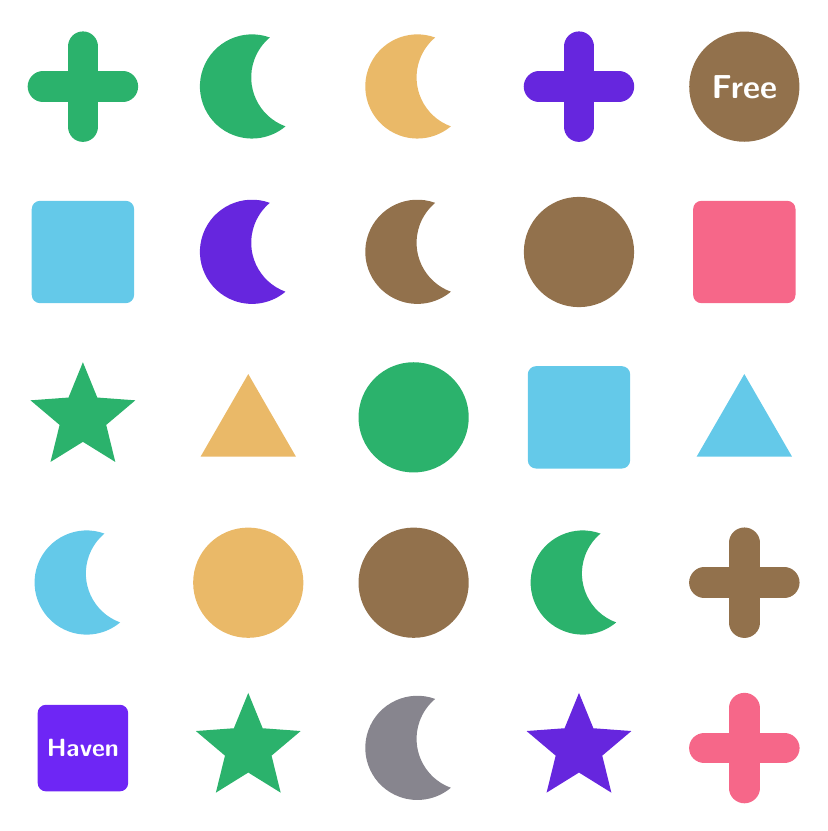
\begin{tikzpicture}[scale=2.1]
    % Definitions
    \definecolor{start-purple}{RGB}{110, 38, 245}
    \definecolor{goal-blue}{RGB}{95, 203, 219}
    \definecolor{green-tone}{RGB}{43, 178, 108}
    \definecolor{gold-tone}{RGB}{234, 185, 104}
    \definecolor{purple-tone}{RGB}{102, 38, 222}
    \definecolor{blue-tone}{RGB}{100, 201, 233}
    \definecolor{brown-tone}{RGB}{146, 113, 76}
    \definecolor{pink-tone}{RGB}{246, 103, 137}
    \definecolor{grey-tone}{RGB}{135, 133, 142}

    \newcommand{\drawmoon}[3]{
        \begin{scope}[shift={(#1)}, rotate=#3, scale=0.9]
            \fill[#2] (0.2,0.3) arc (60:300:0.35) arc
                (240:120:0.35) -- cycle;
        \end{scope}
    }

    \newcommand{\drawplus}[2]{
        \begin{scope}[shift={(#1)}, scale=1.1]
            \draw[line width=11pt, line cap=round, #2]
                (-0.22,0) -- (0.22,0);
            \draw[line width=11pt, line cap=round, #2]
                (0,-0.22) -- (0,0.22);
        \end{scope}
    }

    % Row 1
    \drawplus{0,4}{green-tone}
    \drawmoon{1,4}{green-tone}{10}
    \drawmoon{2,4}{gold-tone}{10}
    \drawplus{3,4}{purple-tone}
    \node[circle, fill=brown-tone, text=white,
          minimum size=1.4cm, inner sep=0
    ] at (4,4) {\large \textsf{\textbf{Free}}};

    % Row 2
    \node[rectangle, fill=blue-tone, rounded corners=3pt,
          minimum size=1.3cm
    ] at (0,3) {};
    \drawmoon{1,3}{purple-tone}{10}
    \drawmoon{2,3}{brown-tone}{10}
    \node[circle, fill=brown-tone, minimum size=1.4cm]
        at (3,3) {};
    \node[rectangle, fill=pink-tone, rounded corners=3pt,
          minimum size=1.3cm
    ] at (4,3) {};

    % Row 3
    \node[star, star points=5, fill=green-tone,
          minimum size=1.4cm, star point ratio=2.25
    ] at (0,2) {};
    \node[regular polygon, regular polygon sides=3,
          fill=gold-tone, minimum size=1.4cm, yshift=-0.15cm
    ] at (1,2) {};
    \node[circle, fill=green-tone, minimum size=1.4cm]
        at (2,2) {};
    \node[rectangle, fill=blue-tone, rounded corners=3pt,
          minimum size=1.3cm
    ] at (3,2) {};
    \node[regular polygon, regular polygon sides=3,
          fill=blue-tone, minimum size=1.4cm, yshift=-0.15cm
    ] at (4,2) {};

    % Row 4
    \drawmoon{0,1}{blue-tone}{10}
    \node[circle, fill=gold-tone, minimum size=1.4cm]
        at (1,1) {};
    \node[circle, fill=brown-tone, minimum size=1.4cm]
        at (2,1) {};
    \drawmoon{3,1}{green-tone}{10}
    \drawplus{4,1}{brown-tone}

    % Row 5
    \node[rectangle, fill=start-purple, rounded corners=3pt,
          minimum size=1.1cm, text=white
    ] at (0,0) {\small \textsf{\textbf{Haven}}};
    \node[star, star points=5, fill=green-tone,
          minimum size=1.4cm, star point ratio=2.25
    ] at (1,0) {};
    \drawmoon{2,0}{grey-tone}{10}
    \node[star, star points=5, fill=purple-tone,
          minimum size=1.4cm, star point ratio=2.25
    ] at (3,0) {};
    \drawplus{4,0}{pink-tone}
\end{tikzpicture}
\caption*{Shape Maze Inspired By
\href{https://jrmf.org/wp-content/uploads/Shape-Mazes-Activity-Guide.pdf}
{Julia Robinson Mathematics Festival}
}
\end{figure}


\section{Farmer's Problems}
\begin{enumerate}[itemsep=1.8em]
% Problem 1
\item
What is the number of possible words that can form
with the letters H, A, V, E, N?

$
\textbf{(A) } 60  \qquad
\textbf{(B) } 120 \qquad
\textbf{(C) } 25  \qquad
\textbf{(D) } 5
$

% Problem 2
\item
Possible words with B, A, N, A, N, A??

$
\textbf{(A) } 36  \qquad
\textbf{(B) } 120 \qquad
\textbf{(C) } 720 \qquad
\textbf{(D) } 60
$

% Problem 3
\item
The notorious farmer needs some help with counting!
How many integers between $1000$ and $9999$ have four
distinct digits?

$
\textbf{(A) } 4536 \qquad
\textbf{(B) } 3024 \qquad
\textbf{(C) } 5040 \qquad
\textbf{(D) } 6480
$

% Problem 4
\item
This time, the farmer wants to know the probability
that a randomly chosen integer between $1000$ and $9999$
is an odd integer whose digits are all distinct!

$
\textbf{(A) } \frac{107}{400} \qquad
\textbf{(B) } \frac{14}{75}   \qquad
\textbf{(C) } \frac{56}{225}  \qquad
\textbf{(D) } \frac{7}{25}
$

% Problem 5
\item
The farm animals love the number $2$. Therefore, the
farmer decided to count the number of integers between
$100$ and $400$ that contains the number $2$. Can you
help him with the counting?

$
\textbf{(A) } 100 \qquad
\textbf{(B) } 138 \qquad
\textbf{(C) } 140 \qquad
\textbf{(D) } 148
$

% Problem 6
\item
Swanky the donkey had a beef with the farmer due to low
compensation for work. Swanky, being a swanky donkey,
offered a mathematical game to the farmer to demand
an increase in ``celery''. The rule is simple. The
farmer is given a fair coin where he flips the coin
in every turn. If the coin lands on tails, the farmer
moves one step to the left. Where as if the coin
lands on heads, the farmer moves one step to the right.

The farm has a fence at position $x = 0$ and a
garden of nuggets at position $x = 10$. If the farmer
ever hits the fence, he loses, and Swanky receives
the raise. On the other hand, Swanky loses if the
farmer reaches the nugget garden.

What is the probability that the farmer loses if
he starts from position $x = 4$?

$
\textbf{(A) } \frac{1}{2} \qquad
\textbf{(B) } \frac{1}{3} \qquad
\textbf{(C) } \frac{2}{5} \qquad
\textbf{(D) } \frac{9}{25}
$

% Problem 7
\item
Hmmm... Swanky is still not satisfied with the
probability. This time, Swanky decided to give the
farmer an unfair coin with $p = 0.6$ as the probability
of landing on tails. Swanky being swanky, he decided
to move the garden of nuggets to $x = 1000$.

If the farmer start from the position $x = 600$,
what is the probability that Swanky receives the raise?

$
\textbf{(A) } 0.6          \qquad
\textbf{(B) } 1 - \epsilon \qquad
\textbf{(C) } 0.36         \qquad
\textbf{(D) } 1
$

% Problem 8
\item
After losing the game with Swanky, the notorious
farmer decided to study probability. Can you help
him find the probability of rolling a fair die six
times and getting at least a five at least five times?

$
\textbf{(A) } \frac{2}{729}  \qquad
\textbf{(B) } \frac{3}{729}  \qquad
\textbf{(C) } \frac{12}{729} \qquad
\textbf{(D) } \frac{13}{729}
$
\end{enumerate}


\section{Solutions}
Solutions available
\href{https://drive.google.com/file/d/1bC1j62365YgbhzAENrZrXA1RmlCdEhc-/view?usp=sharing}{here}!!


\section{Resources Consulted}
\begin{itemize}
\item
Shape Maze Motivation:
\href{https://jrmf.org/wp-content/uploads/Shape-Mazes-Activity-Guide.pdf}
{Julia Robinson Mathematics Festival}

\item
Problem 3: 2015 AMC 8 Problem 10
\item
Problem 4: 2017 AMC 8 Problem 20
\item
Problem 5: 1985 AJHSME Problem 15
\item
Problem 8: 1974 AHSME Problem 24
\end{itemize}

\end{document}

